\chapter{Analytical Model and Preliminary Results}
In this chapter first a framework for the analysis that is performed is presented, later the basic model that is used for the analysis is presented and later calibrated and verified with experimental data available in the literature. Finally preliminary results are presented that will define the general view for the proposed research

\section{Analytical Model}

This study focuses on the behavior of a Single Degree of Freedom Reinforce Concrete Column. The column is modeled as a cantilever structure as shown in \fref{}

\section{Analytical Framework}

An overall analytical framework is stablished such that several analysis can be performed. From this analysis it is possible to determine the effects of damage in the performance of structures. The proposed analytical framework consists in:

\begin{enumerate}
	\item Geometrical Properties of the SDOF column 
	\item Properties of the material are evaluated (i.e. water to cement ratio, cover)
	\item For equal periods of time the Time Dependent Properties are modified
	\item Nonlinear Time History Analysis are performed for discrete events or sequence of events
	\item Results are obtained and evaluated
\end{enumerate}

This procedure has been sumarized in the form of a flow chart presented in \fref{fig:NLTHA_Framework}

\begin{figure}[htbp]
	\centering
	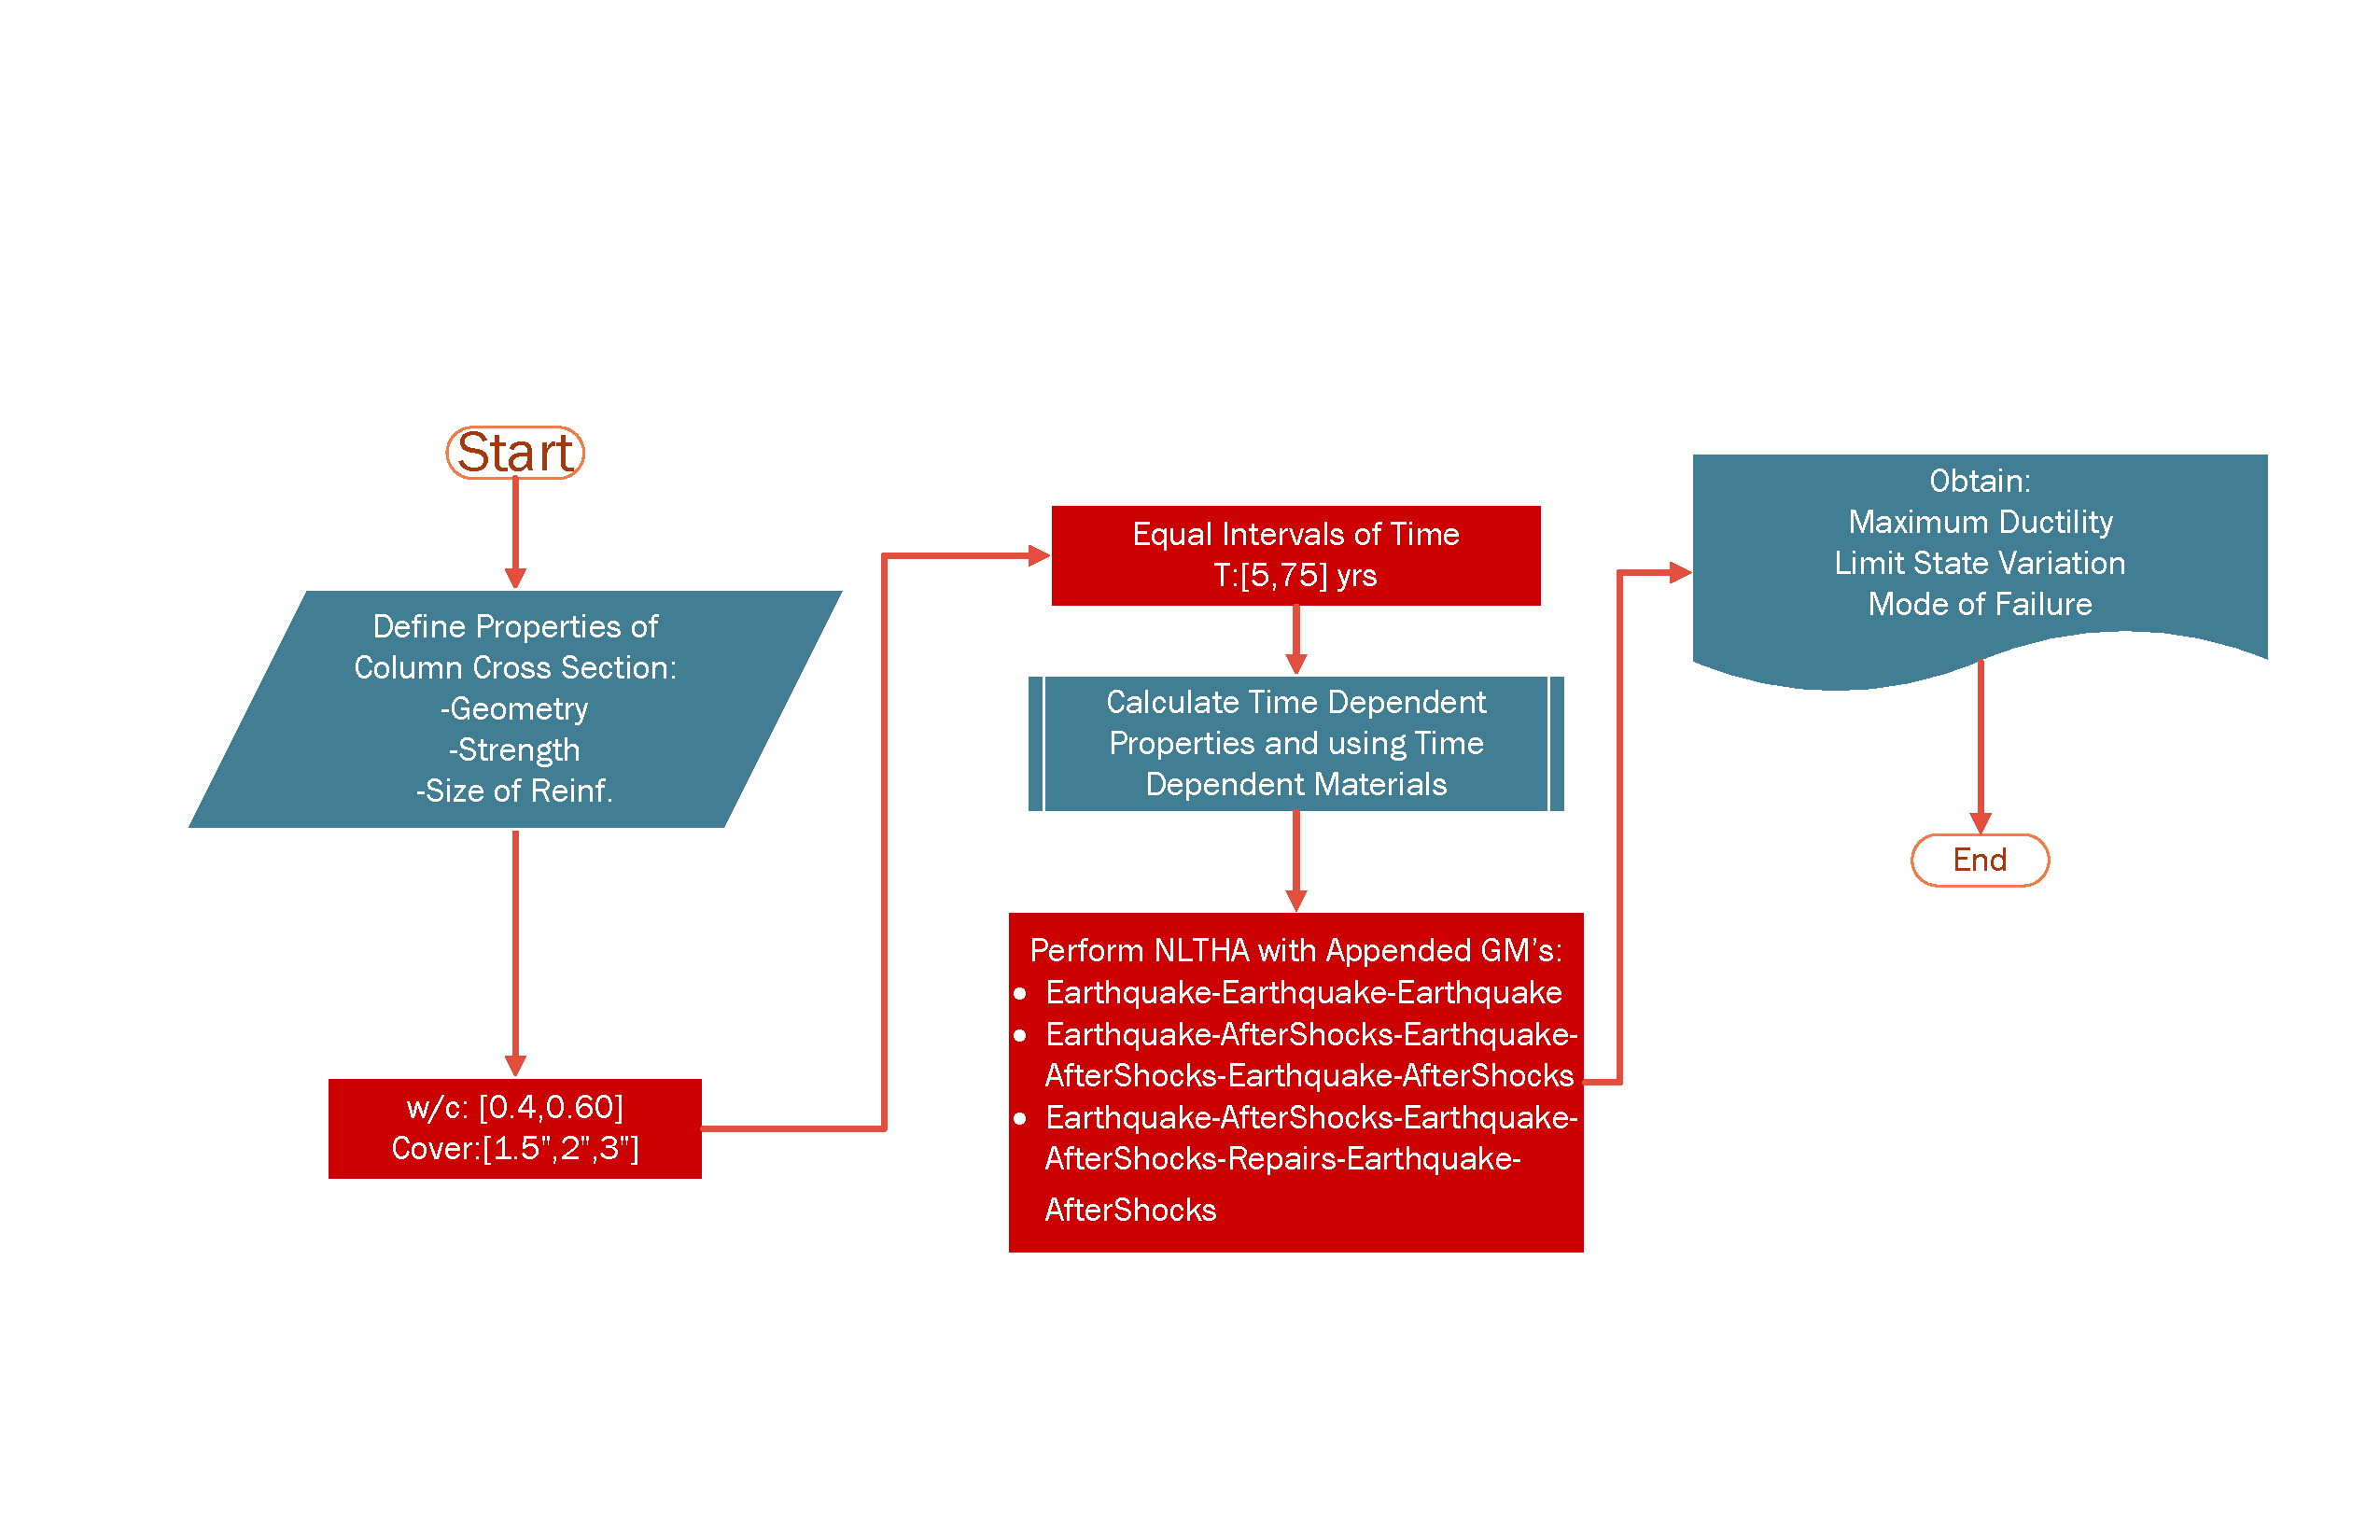
\includegraphics[width=0.9\textwidth]{Chapter-5/figs/AnalysisFramework_01}
	\caption{Analysis Framework Flowchart}
	\label{fig:NLTHA_Framework}
\end{figure}

\section{Model Calibration}
\lipsum[2]
\section{Comparison with existing physical Tests}
\lipsum[3]
\section{Earthquake selection}
\lipsum[4]
\section{Results from NLTHA}
\lipsum[5]
\subsection{Effect on global response}
\lipsum[6]
\subsection{Effect on local response}
\lipsum[7]
\subsection{Preliminary results}
\lipsum[8]